\documentclass[letterpaper]{article} % DO NOT CHANGE THIS
\usepackage[submission]{aaai2027}  % DO NOT CHANGE THIS
\usepackage[hyphens]{url}  % DO NOT CHANGE THIS
\usepackage{graphicx} % DO NOT CHANGE THIS
\urlstyle{rm} % DO NOT CHANGE THIS
\def\UrlFont{\rm}  % DO NOT CHANGE THIS
\usepackage{natbib}  % DO NOT CHANGE THIS AND DO NOT ADD ANY OPTIONS TO IT
\usepackage{caption} % DO NOT CHANGE THIS AND DO NOT ADD ANY OPTIONS TO IT
\frenchspacing  % DO NOT CHANGE THIS
\usepackage{booktabs}
\usepackage{amsmath}
\usepackage{amsthm}
\newtheorem{proposition}{Proposition}
\newtheorem{lemma}{Lemma}
\newtheorem{theorem}{Theorem}
\pdfinfo{
/TemplateVersion (2027.1)
}
\setcounter{secnumdepth}{1}

\title{Supplementary Material:\\A Controlled Study of Attention-Only Transformers}
\author{
    Anonymous Submission
}
\affiliations{
}

\begin{document}
\maketitle

\section{Formal Statements and Proofs}

Notation: one block at position $i$ computes
$y_i = x_i + \sigma(g)\,W_o \sum_j A_{ij}(x)\,W_v \hat u_j$, with
$\hat u = \mathrm{diag}(1+\gamma)\,x/\rho(x)$, $\rho(x)=\mathrm{RMS}(x)$,
and $A$ row-stochastic (softmax over the causal, document-masked scores).

\begin{proposition}[Conditional linearity]
For any fixed row-stochastic $A$, the map
$(\hat u_1,\dots,\hat u_T)\mapsto(\Delta_1,\dots,\Delta_T)$ is linear.
\end{proposition}
\begin{proof}
It is the composition of the linear maps $W_v$, $v\mapsto Av$, and $W_o$,
scaled by the constant $\sigma(g)$.
\end{proof}

\begin{proposition}[Simplex transport]
Per head, the pre-projection update $\sum_j A_{ij}(W_v\hat u_j)$ lies in
the convex hull of $\{W_v \hat u_j : j \le i\}$.
\end{proposition}
\begin{proof}
Softmax rows are nonnegative and sum to 1.
\end{proof}
A head transports content present in context; it does not leave the convex
hull of transformed context vectors. This is the formal sense in which the
main text's ``context-grounded'' interpretation is used, and its
contrapositive is the mechanism behind the distribution-relative task
identity discussed there: when a task's answer is supported by
in-distribution context, transport suffices.

\begin{lemma}[Scalar bottleneck at $T=1$]
For sequence length 1, $A=[1]$ and RoPE at position 0 is the identity, so
each block reduces to $x_{\ell+1} = (I + \tilde B_\ell/\rho_\ell)\,x_\ell$
with $\tilde B_\ell = \sigma(g_\ell)\,W_o W_v\,\mathrm{diag}(1+\gamma_\ell)$
constant and $\rho_\ell = \mathrm{RMS}(x_\ell)$. Hence
$x_L = \big[\prod_\ell (I + \tilde B_\ell/\rho_\ell)\big]x_0$: the entire
depth-$L$ network is a linear map modulated by exactly $L$ scalars.
\end{lemma}
\begin{proof}
Induction on $\ell$; each factor is constant given $\rho_\ell$, which is a
scalar function of $x_\ell$.
\end{proof}
Corollaries: restricted to any sphere $\|x_0\|=r$ the first block is
linear, and any two inputs with identical radius trajectories are
processed by the same linear map. All per-position nonlinearity in a SAN
flows through this $L$-scalar bottleneck; cross-token attention is the
only escape.

\begin{theorem}[Bounded stream variance at initialization]
Assume the initialization as implemented: $\gamma=0$ (norms are exact RMS
normalizations), gates $\sigma(0)=\tfrac12$, $W_o$ entries i.i.d.\
mean-zero with variance $s^2/(2N)$, $W_v$ fixed-scale, all independent.
Then for every depth $N$,
$\mathbb{E}\|x_N\|^2 = \mathbb{E}\|x_0\|^2 + \sum_\ell
\mathbb{E}\|b_\ell\|^2$ with $\mathbb{E}\|b_\ell\|^2 = \Theta(1/N)$, hence
$\mathbb{E}\|x_N\|^2 = \mathbb{E}\|x_0\|^2 + \Theta(1)$ uniformly in $N$.
\end{theorem}
\begin{proof}
Cross terms $\mathbb{E}\langle x_\ell, b_\ell\rangle$ vanish because $W_o$
is mean-zero and independent of everything upstream. Each branch input is
RMS-normalized, so $\mathbb{E}\|z_\ell\|^2$ is bounded independent of the
stream magnitude; row-stochastic $A$ cannot increase the maximum value
norm (Proposition 2); the $1/(2N)$ output variance then gives
$\mathbb{E}\|b_\ell\|^2 = \Theta(1/N)$, and the sum telescopes.
\end{proof}
Each hypothesis is load-bearing: drop the $1/\sqrt{2N}$ scaling or the
gate and the sum is $\Theta(1)$ per layer, $\Theta(N)$ total; drop
pre-norm and growth compounds. Empirically (main text), trainability to 48
layers held, but the gate factor proved dispensable: standard residuals
match gated ones at every depth tested, so the initialization scaling and
normalization carry the result.

\begin{proposition}[Weight-decay fixed point of norm gains]
Under $L_2$ decay, the penalty on $\gamma$ in the $(1+\gamma)$
parameterization is minimized at gain 1 (identity); under the standard
parameterization (gain $h$, init 1) it is minimized at $h=0$, the zero
map.
\end{proposition}
\begin{proof}
Both objectives are strictly convex with the stated minimizers.
\end{proof}
In our fixed frame, weight decay applies to kernels only, so the two
parameterizations are additionally \emph{optimizer-equivalent} (they
differ by a constant shift, and Adam-family updates are shift-invariant).
Training both anyway yielded $\Delta = 0.0015$ nats, which we use as the
study's same-seed noise floor.

\begin{lemma}[Muon bounds per-step spectral drift, and only that]
Let the update be $\Delta = -\eta P$ with $P$ the polar factor of the
momentum gradient (Newton--Schulz approximation error $\varepsilon$). By
Weyl's inequality for singular values, for every $i$,
$|\sigma_i(W+\Delta)-\sigma_i(W)| \le \|\Delta\|_2 = \eta(1+\varepsilon)$.
After $t$ steps every singular value lies within $t\eta$ of its
initialization.
\end{lemma}
This bounds drift; it does not prove spectra stay balanced nor that
balance improves loss. The measured outcome (main text) is that Muon
holds routing-matrix spectra 2--3$\times$ flatter than AdamW in both
architectures, i.e.\ the effect is real but not architecture-differential.

\section{Pre-Registration and Scorecard}

All hypotheses and predictions were registered in the project repository
on 2026-07-14, before the corresponding measurements; the fineweb-edu
prediction was registered numerically on 2026-07-19, before that run was
launched. Registered predictions and outcomes:

\begin{table}[h]\centering\small
\begin{tabular}{p{0.12\columnwidth}p{0.78\columnwidth}}
\toprule
P1 & \textbf{Confirmed.} Iso-param gap within the seed band at 105B
(clean pairs $+0.0055/+0.0054$). \\
P2 & \textbf{Confirmed at 31B} (trace gap smallest); at 105B trace and
answer both reach parity, superseded by full localization. \\
P3 & \textbf{Falsified as stated.} The gap peaks on low-context query
tokens, not memorization answers; the restated account then made the
confirmed fineweb prediction. \\
P4 & \textbf{Gates component falsified} by its own criterion (gated
$\approx$ ungated everywhere); trainability confirmed; QK-norm emerged,
unpredicted, as the load-bearing component. \\
P5 & \textbf{Not exercised}: the fixed frame decays kernels only; the
measurement instead calibrated the noise floor (0.0015). \\
P6 & \textbf{Budget-dependent}: full optimizer$\times$architecture
crossover at 5B; gone by 30B. \\
P7 & \textbf{Half-confirmed}: spectra flatter under Muon everywhere, but
not differentially in the SAN; representation rank high everywhere
(minimum 173/512 at 20 layers). \\
P8 & \textbf{Falsified}: no architecture$\times$repetition interaction;
both arms nearly repetition-insensitive to 18 epochs. \\
\bottomrule
\end{tabular}
\caption{Registered predictions vs.\ outcomes. The instruments were
designed so that predictions could fail; two did, and one failure produced
the paper's central finding.}
\end{table}

\section{Learning-Rate Fairness Sweep}

Each arm$\times$optimizer cell received a 3-point sweep
(0.5$\times$/1$\times$/2$\times$) at 5B tokens with a boundary rule: any
sweep-edge winner was extended by another doubling until its curve turned
(17 cells total). Final losses and locks:

\begin{table}[h]\centering\small
\begin{tabular}{lccccccl}
\toprule
Arm & 0.5$\times$ & 1$\times$ & 2$\times$ & 4$\times$ & 8$\times$ &
16$\times$ & Lock \\
\midrule
SAN Muon & 2.248 & \textbf{2.245} & 2.251 & & & & 0.02 \\
FFN Muon & 2.223 & 2.224 & \textbf{2.216} & 2.237 & & & 0.04 \\
SAN AdamW & 2.361 & 2.293 & \textbf{2.267} & 2.321 & & & 6e-4 \\
FFN AdamW & 2.305 & 2.254 & 2.230 & 2.219 & \textbf{2.199} & 2.216 &
2.4e-3 \\
\bottomrule
\end{tabular}
\caption{All four locks are interior minima. At the most extreme rate
(16$\times$), the FFN model's FFN gates collapsed to mean 0.07 while its
attention gates stayed structured: under learning-rate stress the standard
transformer self-pruned toward attention-only form and still reached
2.216.}
\end{table}

At 30B tokens with the locked rates, the optimizer$\times$architecture
crossover visible at 5B has washed out entirely:

\begin{table}[h]\centering\small
\begin{tabular}{lcc}
\toprule
@30B tokens & Muon & AdamW \\
\midrule
SAN 24M & 2.1126 & 2.1103 \\
FFN iso-param 24M & 2.0933 & 2.0950 \\
\bottomrule
\end{tabular}
\caption{The optimizer 2$\times$2 at 30B: within-architecture deltas are
$\le 0.002$ nats (vs.\ 0.022/0.017 crossover at 5B). The interaction is a
short-horizon phenomenon.}
\end{table}

Ladder learning-rate probes: before interpreting the size ladder, 3-point
rate probes (0.5$\times$/1$\times$/2$\times$ of the lock, 2.5k-step
horizon) at the smallest and largest sizes confirmed the transferred lock
is in the flat region at tiny (2.851/2.856/2.857) and an interior minimum
at xl (2.074/2.066/2.078); no per-size sweeps were needed.

\section{Full Downstream Results}

% Supplementary: full 0-shot downstream results
\begin{table*}[t]\centering\small
\begin{tabular}{lccccccc}
\toprule
Model & lambada (ppl) & sciq & arc\_easy & piqa & hellaswag & winogrande & mmlu \\
\midrule
chance & $\sim$0 & 0.25 & 0.25 & 0.50 & 0.25 & 0.50 & 0.25 \\
\midrule
SAN 24M @31B & 0.091 (821) & 0.725 & 0.397 & 0.545 & 0.279 & 0.504 & 0.236 \\
FFN iso-param 24M @31B & 0.136 (492) & 0.702 & 0.416 & 0.563 & 0.283 & 0.516 & 0.233 \\
SAN 24M @105B (3-seed mean) & 0.111 (682) & 0.742 & 0.405 & 0.559 & 0.284 & 0.517 & 0.232 \\
FFN iso-param 24M @105B (3-seed mean) & 0.134 (518) & 0.661 & 0.415 & 0.558 & 0.283 & 0.511 & 0.245 \\
FFN iso-FLOP 43M @105B & 0.178 (451) & 0.634 & 0.419 & 0.562 & 0.293 & 0.534 & 0.230 \\
FFN iso-depth 87M @105B & 0.111 (964) & 0.630 & 0.426 & 0.552 & 0.288 & 0.525 & 0.233 \\
SAN 24M fineweb-trained @31B & 0.203 (189) & 0.705 & 0.447 & 0.579 & 0.294 & 0.507 & 0.231 \\
FFN iso-param fineweb-trained @31B & 0.181 (218) & 0.707 & 0.478 & 0.588 & 0.287 & 0.507 & 0.232 \\
\bottomrule
\end{tabular}
\caption{Complete 0-shot results. Note the capacity axis at 105B: iso-FLOP
(43M) improves lambada over iso-param (24M) but iso-depth (87M), the best
in-distribution model, is the worst at out-of-distribution recall
(lambada 0.111, ppl 964) and sciq drops monotonically with FFN capacity
(0.702/0.634/0.630): in-distribution capacity over-specializes.}
\label{tab:downstream_full}
\end{table*}


Two capacity-axis observations. Out-of-distribution recall (lambada) is
non-monotone in FFN capacity: iso-FLOP (43M) improves over iso-param
(24M), but iso-depth (87M), the best in-distribution model, is the worst
(acc 0.111, ppl 964). Sciq falls monotonically with FFN capacity
(0.702/0.634/0.630) while the SAN improves with training (0.725
$\rightarrow$ 0.742): in-distribution capacity over-specializes, and
context-faithfulness erodes as parametric priors strengthen.

\section{Repetition and Data Scaling}

\begin{figure}[h]
\centering
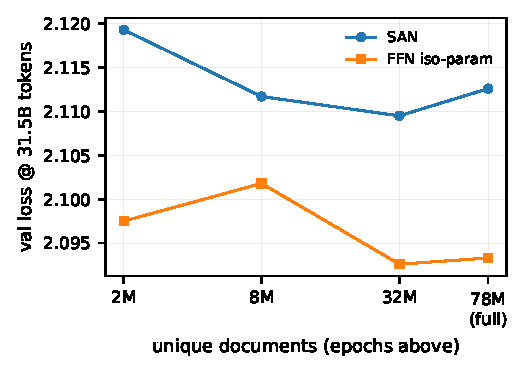
\includegraphics[width=0.9\columnwidth]{Figures/fig6_e5_suppl.pdf}
\caption{Constraining unique documents at a fixed 31.5B-token budget.
Both arms are nearly repetition-insensitive (18 epochs cost $\le 0.010$
nats), with no architecture interaction.}
\end{figure}

\section{Gate Trajectories and FFN-Arm Observations}

\begin{figure}[h]
\centering
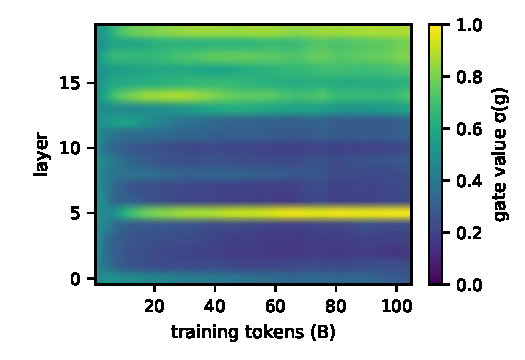
\includegraphics[width=0.9\columnwidth]{Figures/fig5_gates_suppl.pdf}
\caption{Gate values over training, SAN 105B run (layers $\times$ time).
Early layers self-attenuate and late layers sharpen under Muon.}
\end{figure}

Although performance-neutral, the gates were diagnostically productive.
Three independent observations of FFN-arm fragility: (i) at 16$\times$ the
tuned rate, all FFN gates collapsed (mean 0.07) while attention gates
stayed structured; (ii) at the tuned rate under Muon, FFN gates ended low
(mean 0.16--0.17) in three separate runs, echoing the same self-pruning;
(iii) one of three FFN seeds at 105B suffered a terminal-phase
instability, its gradient norm tripling over the final 800 steps at the
learning-rate floor (Figure~\ref{fig:tail}); no SAN run showed any of
these behaviors. We report these as observations, not claims.

\begin{figure}[h]
\centering
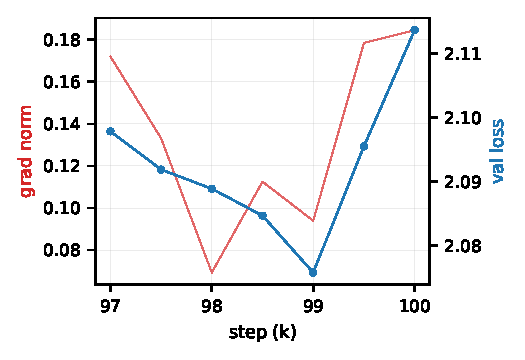
\includegraphics[width=0.9\columnwidth]{Figures/fig8_s43_tail_appendix.pdf}
\caption{The FFN iso-param seed-43 terminal instability. The run tracked
its sibling seed to within 0.002 nats through step 99{,}000. Its final
value is included, flagged, in all statistics.}
\label{fig:tail}
\end{figure}

\section{Depth Ladder}

\begin{figure}[h]
\centering
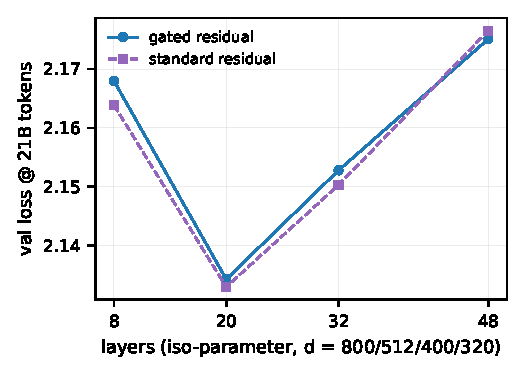
\includegraphics[width=0.9\columnwidth]{Figures/fig7_depth.pdf}
\caption{Iso-parameter depth ladder for the SAN arm, gated vs.\ standard
residuals: U-shaped in depth with a 20-layer optimum; gates neutral at
every depth; 48 layers train without incident.}
\end{figure}

\section{Reproducibility Details}

\textbf{Frame matching.} All headline results use a fixed global batch of
512 rows (64/device $\times$ 8) of 2048 tokens. Phases run on 7-GPU nodes
used 73 rows/device (511 total, $-0.2\%$) with learning rates rescaled so
effective values equal the 8-device locks (Adam scales linearly in device
count, Muon as its square root). A base-size pair rerun across frames
agreed to 0.0033 nats.

\textbf{Determinism and recovery.} Checkpoints store parameters, not
optimizer state. One run was resumed from its 40\%-checkpoint after an
artifact loss; despite cold optimizer state at the stable-phase rate, it
reproduced the original final validation loss exactly (1.5982),
suggesting the warm-restart transient is fully absorbed by the
learning-rate decay phase.

\textbf{Statistics.} Headline comparisons use three seeds per arm with
paired per-seed differences; the same-seed noise floor (0.0015 nats) comes
from the optimizer-equivalent normalization pair. Per-block losses were
not retained, so block-level bootstrap intervals are not reported;
seed-level agreement (clean pairs matching to $10^{-4}$) is the operative
evidence.

\textbf{Artifacts.} Code, tokenizer, corpus tokenization manifests, all
checkpoints with 25\% milestones, training logs, and every evaluation
report will be released upon publication.

\input{ReproducibilityChecklist}

\end{document}
